\documentclass[aspectratio=169,12pt]{beamer}

\usepackage{hyperref}
\usepackage[giveninits=true,doi=false,isbn=false,url=false,eprint=false]{biblatex}



\renewbibmacro*{booktitle}{%
  \textbf{\printfield[booktitle]{booktitle}}%
}


\usepackage{amsmath}
\usepackage{bm}

\usepackage{tcolorbox}

\addbibresource{references.bib}
\addbibresource{publications_oral.bib}

\usepackage{varwidth}
\usepackage{tikz}
\usetikzlibrary{tikzmark}



\tikzset{
    blueblock/.style = {draw=amethyst,thick,fill=amethyst!15,rounded corners=0pt,inner sep=7pt}
}
\tikzset{
    pinkblock/.style = {draw=amaranth,thick,fill=amaranth!15,rounded corners=0pt,inner sep=7pt}
}

\tikzset{
    widepinkblock/.style = {draw=amaranth,thick,fill=amaranth!15,rounded corners=0pt,inner sep=20pt}
}

\usepackage{multirow}
\usepackage{booktabs}
\usepackage{algorithm}
\usepackage{algpseudocode}


\usepackage{amssymb}% http://ctan.org/pkg/amssymb
\usepackage{pifont}% http://ctan.org/pkg/pifont
\newcommand{\cmark}{\ding{51}}%
\newcommand{\xmark}{\ding{55}}%

\definecolor{darkspringgreen}{rgb}{0.09, 0.45, 0.27}
\definecolor{amaranth}{rgb}{0.9, 0.17, 0.31}
\definecolor{amethyst}{rgb}{0.6, 0.4, 0.95}

\usepackage{enumitem}

% Labels for items in (nested) itemize (uses bullets/characters)
\newcommand\labelitemi{\textcolor{amaranth}{\textbullet}}% bullet
\newcommand\labelitemii{\textcolor{amaranth}{\normalsize\normalfont\bfseries \textendash}}% --
\newcommand\labelitemiii{\textcolor{amaranth}{\textasteriskcentered}}% *
\newcommand\labelitemiv{\textcolor{amaranth}{\textperiodcentered}}% .
\setlist[enumerate,1]{label={\textcolor{amaranth}{\arabic*.}}}


% footnote size
\makeatletter
\newcommand\notsotiny{\@setfontsize\notsotiny\@vipt\@viipt}
\makeatother

\setbeamerfont{footnote}{size=\notsotiny}


\makeatletter
\newcommand{\Pause}[1][]{\unless\ifmeasuring@\relax
\pause[#1]%
\fi}
\makeatother
%%%%%% Template things

% space between paragraphs
\parskip=1em

% title font
\setbeamerfont{title}{size=\LARGE}%, series=\bfseries}
\setbeamerfont{frametitle}{size=\LARGE}%, series=\bfseries}
\setbeamerfont{institute}{size=\normalsize}%, series=\bfseries}

% spacing between frame title and content
\addtobeamertemplate{frametitle}{\vspace*{0.2cm}}{\vspace*{0.5cm}\setcounter{footnote}{0}}

% color
\definecolor{beamer@blendedblue}{rgb}{0.8, 0, 0.34}%{0.44, 0.16, 0.39}

% no navigation
\beamertemplatenavigationsymbolsempty

% slide numbers
\setbeamertemplate{footline}
{
  \hbox{\begin{beamercolorbox}[wd=1\paperwidth,ht=5.25ex,dp=4ex,right]{framenumber}%
      \large \insertframenumber{}~~
    \end{beamercolorbox}}%
  \vskip0pt%
}

% slide numbers
\def\setupappendix{
\setcounter{framenumber}{0}
\setbeamertemplate{footline}
{
  \hbox{\begin{beamercolorbox}[wd=1\paperwidth,ht=5.25ex,dp=4ex,right]{framenumber}%
      \large A-\insertframenumber{}~~
    \end{beamercolorbox}}%
  \vskip0pt%
}
}


% centered titles
\makeatletter
\long\def\beamer@@frametitle[#1]#2{%
  \beamer@ifempty{#2}{}{%
    \gdef\insertframetitle{\centering{#2\ifnum\beamer@autobreakcount>0\relax{}\space\usebeamertemplate*{frametitle continuation}\fi}}%
  \gdef\beamer@frametitle{#2}%
  \gdef\beamer@shortframetitle{#1}%
}%
}
\makeatother

%%%%% Equations

\newcounter{mytn}
\makeatletter
\newcommand{\tmn}[3][]{\stepcounter{mytn}%
\tikzmarknode[Col\the\numexpr\value{mytn}-\mytn@start\relax/.try,inner xsep=2pt,%
minimum height=1.6em,inner sep=2mm,#1]{mytn-\number\value{mytn}}{#2}%
\expandafter\gdef\csname tmn@annot@\number\value{mytn}\endcsname{#3}}
\newenvironment{AnnotatedEquation}{\edef\mytn@start{\number\value{mytn}}%
\begin{equation*}}{\end{equation*}%
\edef\mytn@end{\number\value{mytn}}%
\ifnum\mytn@end>\mytn@start
\begin{itemize}
 \foreach \X in {\the\numexpr\mytn@start+1,...,\mytn@end}
 {\item \tikzmarknode{mytn-annot-\X}{\csname tmn@annot@\X\endcsname}%
   \begin{tikzpicture}[overlay,remember picture]
  \draw[-stealth] (mytn-annot-\X.east) to[out=0,in=-90] (mytn-\X.south);
 \end{tikzpicture}}
\end{itemize}
\fi}
\makeatother
\tikzset{ Col1/.style= {fill=blue!20,anchor=base,rounded corners=2pt},
Col2/.style= {Col1, fill=red!20},
Col3/.style= {Col1, fill=green!20},
Col4/.style= {Col1, fill=yellow!20},
}

% footnotes at end of frame rather than minipage

\makeatletter
\renewrobustcmd{\blx@mkbibfootnote}[2]{%
  \iftoggle{blx@footnote}
    {\blx@warning{Nested notes}%
     \addspace\mkbibparens{#2}}
    {\unspace
     \ifnum\blx@notetype=\tw@
       \expandafter\@firstoftwo
     \else
       \expandafter\@secondoftwo
     \fi
       {\csuse{blx@theendnote#1}{\protecting{\blxmkbibnote{end}{#2}}}}
       {\csuse{footnote}[frame]{\protecting{\blxmkbibnote{foot}{#2}}}}}}
\makeatother

%%%%% INFORMATION

\title{\LARGE Convergence and Linear Speed-Up in Stochastic Federated Learning  \\[0.5em]
%Projet de Recherche : 
\vspace{0em}}
\author{
  Paul Mangold\\[0.5em]
  Workshop Fondation Mathématiques de l'IA
}
\titlegraphic{
}
\institute{}
\date{March 25th, 2025}


%%%%% DOCUMENT

\begin{document}

%% TITLE PAGE

\begin{frame}[plain]
  \vspace{3.5em}
  \titlepage
\end{frame}
\addtocounter{framenumber}{-1}

\begin{frame}[t]{Federated Learning}
% \footfullcite{mangold2020decentralized}$^{,}$\footfullcite{ogier2022flamby}$^{,}$\footfullcite{mangold2024scafflsa}$^{,}$\footfullcite{mangold2025refined}$^{,}$\footfullcite{mangold2025scaffold}}
\vspace{0.5em}
  \begin{minipage}{0.35\linewidth}
    \begin{center}
    \only<1>{    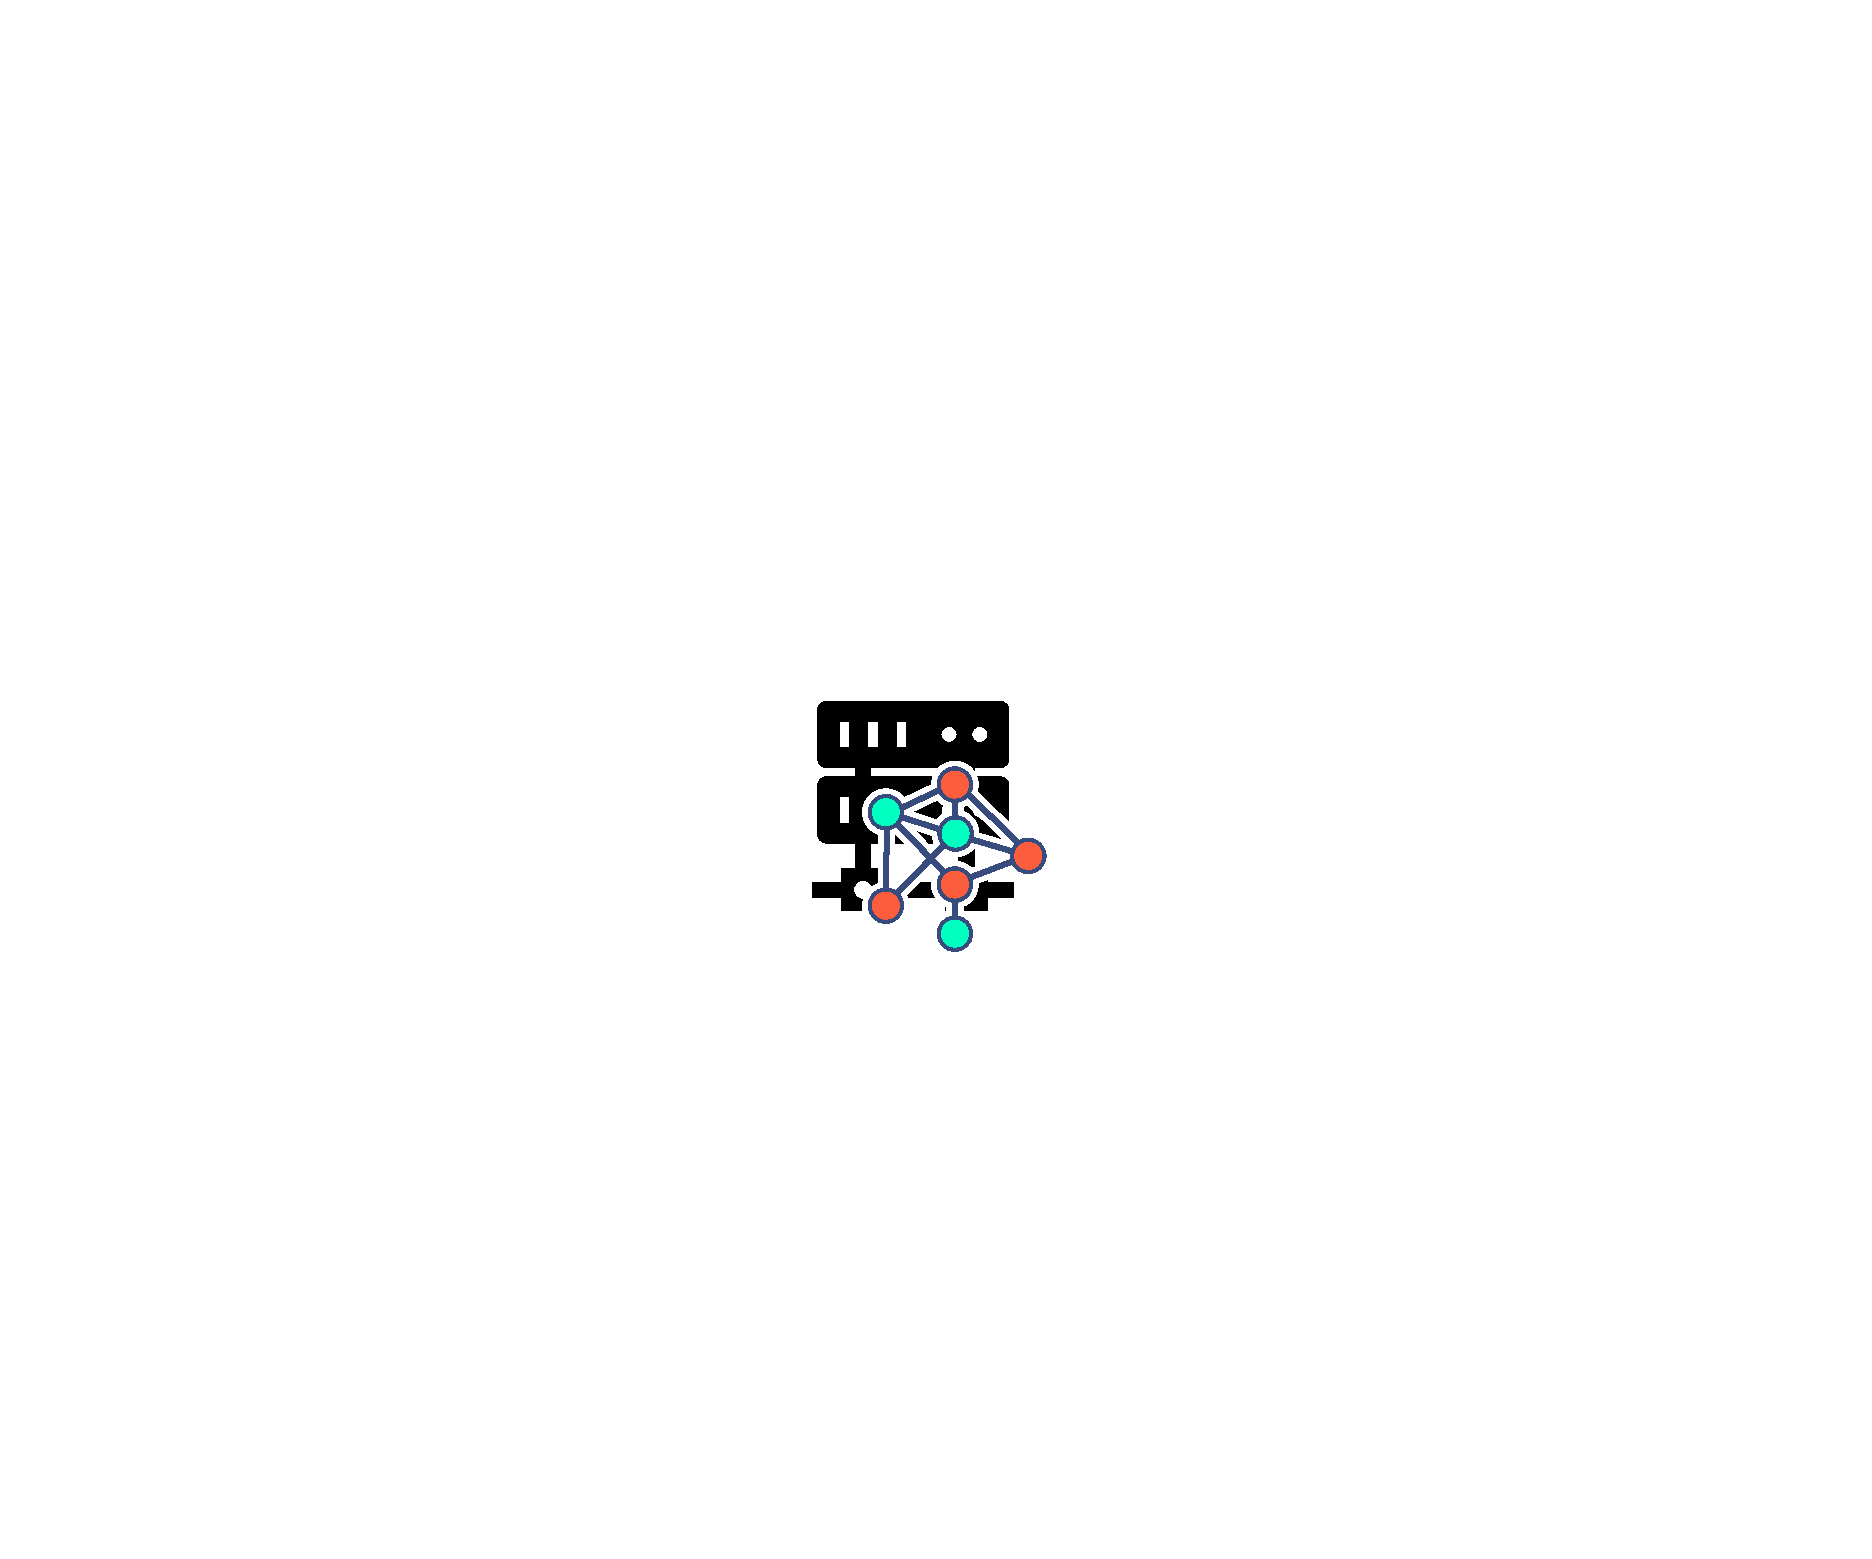
\includegraphics[width=\linewidth]{images/federated_learning_only_server.pdf} }%
    \only<2,3,4>{    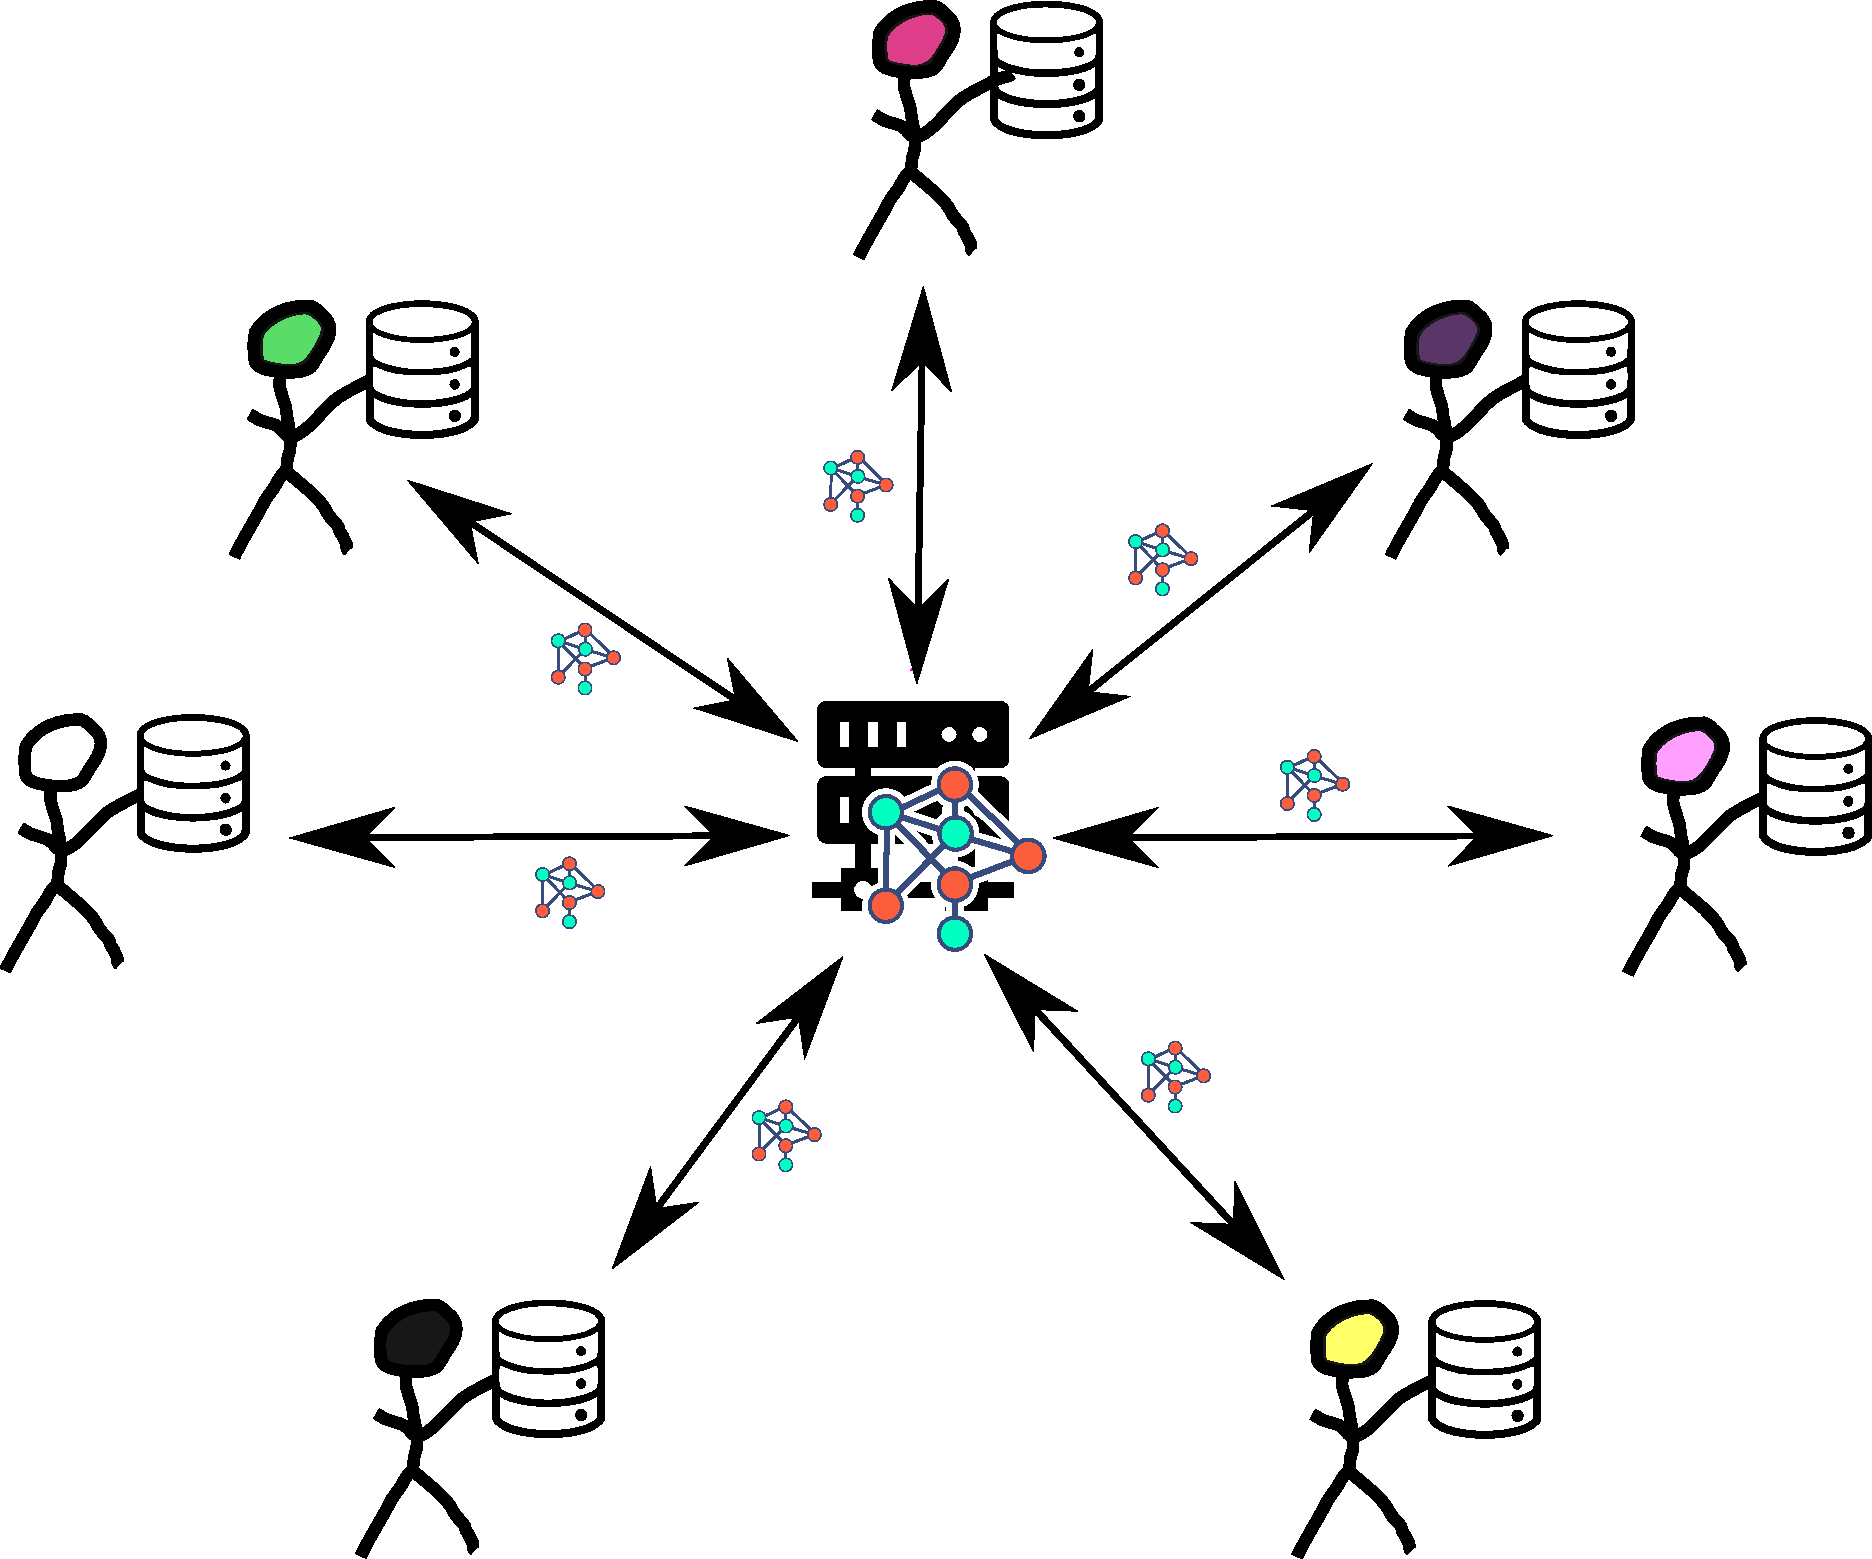
\includegraphics[width=\linewidth]{images/federated_learning.pdf} }
    \end{center}
    
  \end{minipage}~~~~~~%
  \begin{minipage}{0.5\linewidth}

\only<3,4>{
    \begin{center}
      Collaborative optimization problem
      \begin{align*}
        \min_{x \in \mathbb{R}^d} 
        \frac{1}{N} \sum_{c=1}^N f_c(x)
        ~~,
        \quad 
        f_c(x)
        = \mathbb{E}_Z[ F_c(x; Z) ]
      \end{align*}
      % $\rightarrow$ avec une seule \emph{solution globale}
    \end{center}
    }
      
  \end{minipage}

% \vspace{0.5em}

% \only<4>{
%   \begin{center}
%       \textbf{\textcolor{purple}{Difficultés centrales}} : hétérogénéité des données et des moyens de calcul 

%       \vspace{-0.5em}
      
%       + communication lente et difficile à établir
%   \end{center}
% }
  \pause
  \pause
  \pause
  \begin{center}
    \textcolor{purple}{\bfseries Problem: data is heterogeneous, communication is expensive}
  \end{center}
  
\end{frame}



\begin{frame}
  \begin{center}
    \huge \textcolor{purple}{
      I. Federated Averaging
      }
  \end{center}
\end{frame}


\begin{frame}[t]{Federated Averaging\footfullcite{mcmahan2017communicationoral} ~~~ \raisebox{0.2em}{\textcolor{black}{\normalsize $x^\star \in \arg\min_{x \in \mathbb{R}^d} 
    \frac{1}{N} \sum_{c=1}^N \mathbb{E}_Z[ F_c(x; Z) ]$}} ~~}  
    
    \vspace{1em}

  \begin{minipage}{0.5\linewidth}

  \footnotesize
  At each global iteration

    \begin{itemize}[leftmargin=*,itemsep=0em]
  \footnotesize
    \item For $c=1$ à $N$ in parallel

\vspace{-0.2em}
    
    
\begin{itemize}[leftmargin=*,itemsep=0em]
\item Receive $x^{(t)}$, set $x^{(t,0)}_c = x^{(t)}$
    
        \item For $h=0$ to $H-1$
    \end{itemize}

\vspace{-0.6em}
\begin{center}
            \hspace{-1em}$x^{(t,h+1)}_c = x^{(t,h)}_c - \gamma \nabla F_c( x^{(t,h)}_c ; Z_c^{(t,h+1)})$
        \end{center}
      
  \item Aggregate local models 
        
        
\vspace{-0.6em}
\begin{center}
            \hspace{-1em}$x^{(t+1)} = \frac{1}{N} \sum_{c=1}^N x_c^{(t,H)}$
        \end{center}
      
    \end{itemize}
      
  \end{minipage}~%
  \begin{minipage}{0.48\linewidth}
    \pause
    \begin{center}
      \small
    With deterministic gradients:
    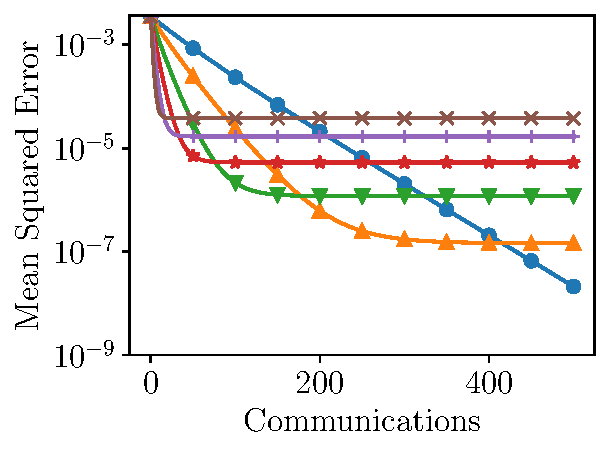
\includegraphics[width=0.75\linewidth]{images/local_training_heterogeneous.pdf}%
    \raisebox{2.5em}{ 
\includegraphics[width=0.25\linewidth]{images/legend.pdf} }
  \end{center}
  
  %   \vspace{-0.5em}

  % ~~~~Plus d'itérations locales

  %   \vspace{0.5em}
    
  %   ~~~~~{\large \textcolor{green} \cmark}\, convergence plus rapide
    
  %   ~~~~~{\large \textcolor{red} \xmark}~ biais plus grand

  \end{minipage}

  \vspace{1.5em}


\end{frame}

\begin{frame}{Classical analyses of this algorithm\\[-0.5em]
    \small (For $L$-smooth, $\mu$-strongly convex functions)}

  Choose your favorite heterogeneity measure
  \begin{itemize}
  \item first-order\footfullcite{lian2017can}: $\zeta = \frac{1}{N} \sum_{c=1}^N \big\| \nabla f_c(x^{\star}) - \nabla f(x^{\star}) \big\|^2$
  \item second-order\footfullcite{khaled2022faster}: $\zeta = \frac{1}{N} \sum_{c=1}^N \big\| \nabla_c^2 f(x^{\star}) - \nabla^2 f(x^{\star}) \big\|^2$
  \item average drift\footfullcite{wang2024Unreasonable}: $\zeta = \big\| \frac{1}{NH} \sum_{c=1}^N \sum_{h=0}^{H-1} \nabla f(x_c^{(h)}) - \nabla f(x^{\star}) \big\|^2$
  \end{itemize}

  \vspace{0.5em}

  \pause

  Show \textcolor{purple}{\bfseries convergence to a neighborhood} of $x^\star$
  \begin{align*}
    \| x^{(T)} - x^\star \|^2 \lesssim (1 - \gamma \mu)^{HT} \| x^{(0)} - x^\star \|^2
    + \textcolor{purple}{\boldsymbol{\chi(\gamma, H, \zeta)}} ~~~~~\text{\small (for some function $\chi$)}
  \end{align*}

  \vspace{1em}

  
\end{frame}


\begin{frame}[t]
  \begin{center}
    
  \resizebox{0.9\linewidth}{!}{
  \begin{tikzpicture}
    \draw [-to,very thick](0,0) -- (12.5,0);
    \node at (1.5,0.2) {$H=2$};
    \node at (6,0.2) {$H=10$};
    \node at (10.5,0.2) {$H=50$};
  \end{tikzpicture}
}
\vspace{-0.5em}

\only<1>{
  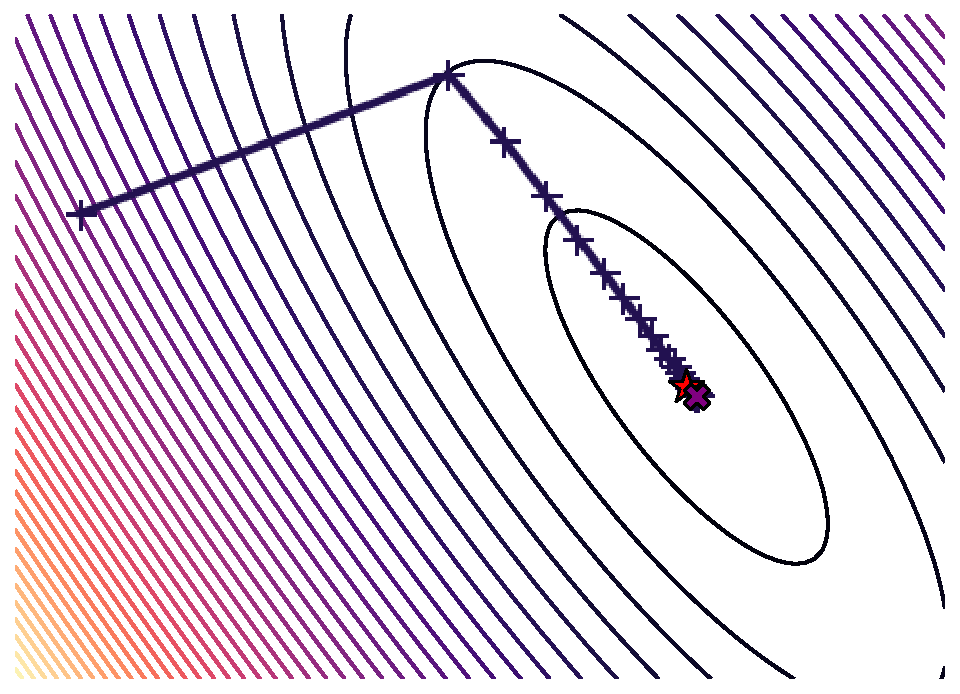
\includegraphics[width=0.3\linewidth]{images/plots/fedavg_False_2_t1000_s0.pdf}
  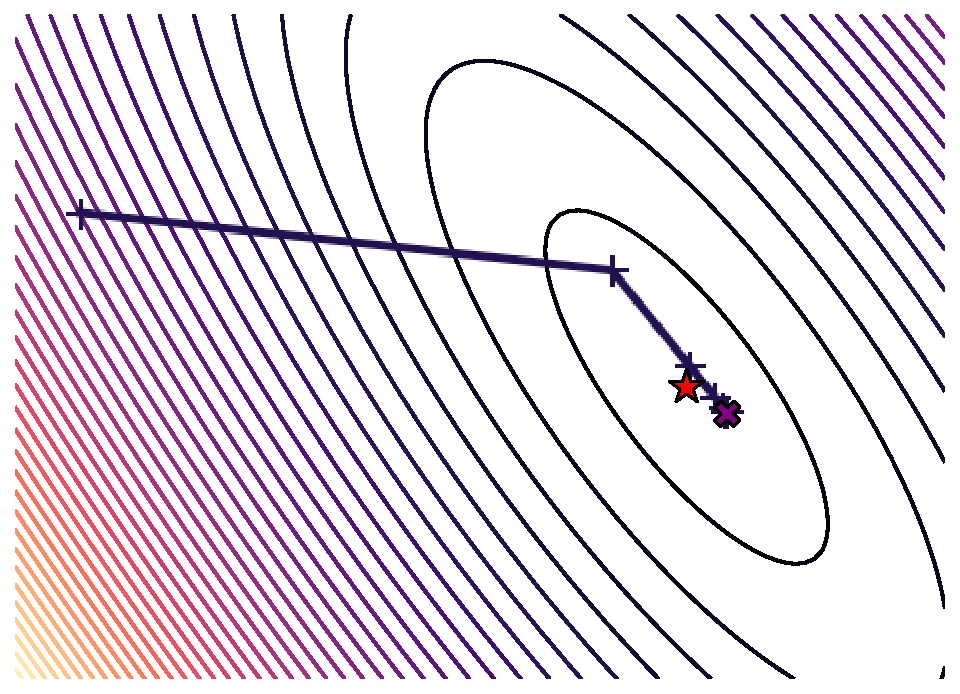
\includegraphics[width=0.3\linewidth]{images/plots/fedavg_False_10_t1000_s0.pdf}
  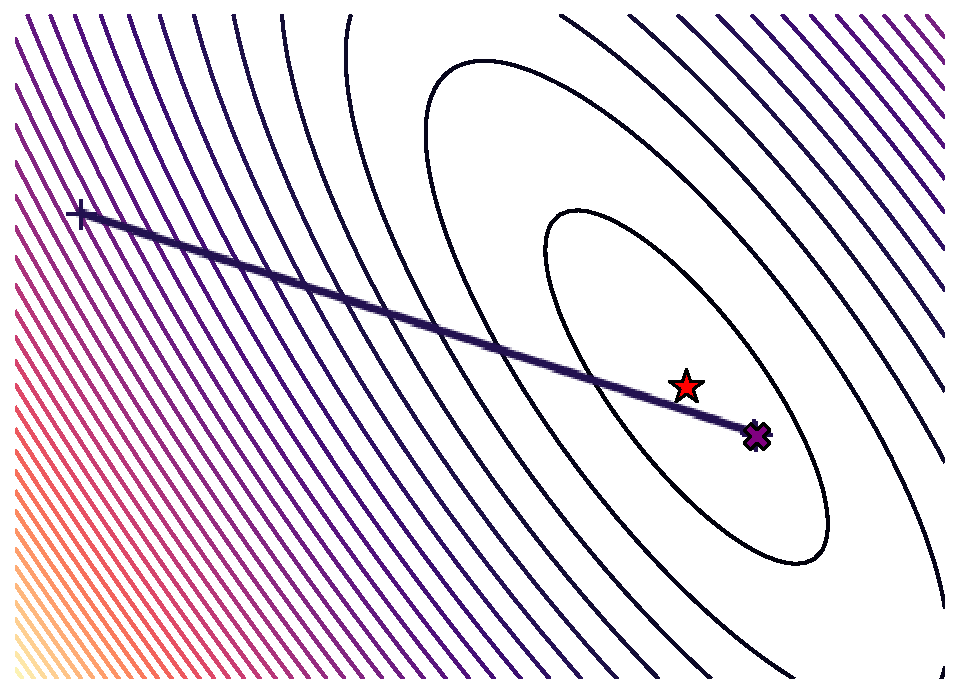
\includegraphics[width=0.3\linewidth]{images/plots/fedavg_False_50_t1000_s0.pdf}
}%
\only<2,3>{
  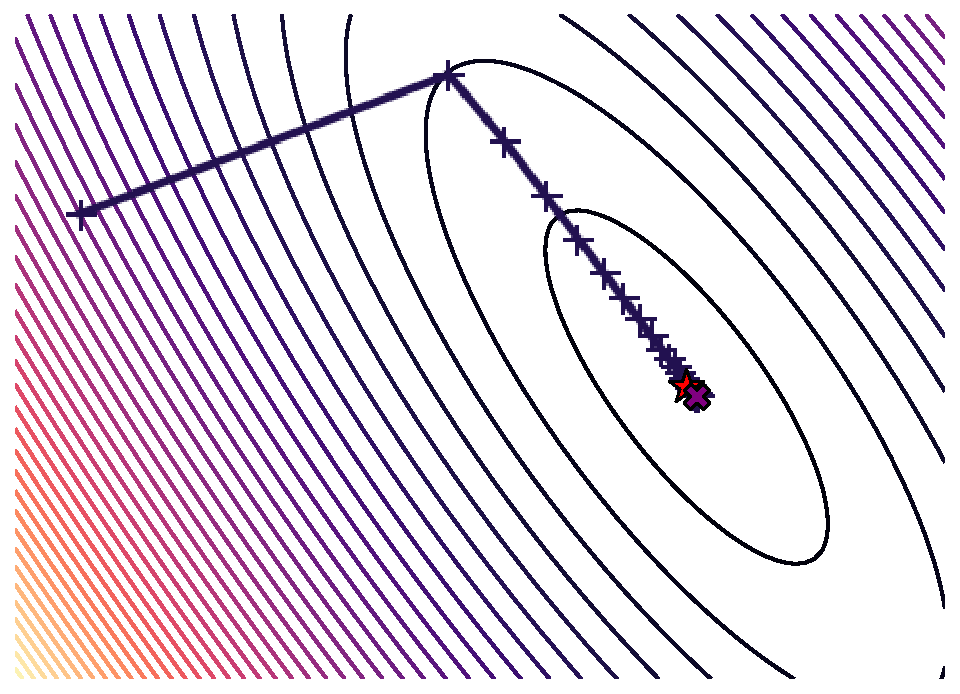
\includegraphics[width=0.3\linewidth]{images/plots/fedavg_True_2_t1000_s0.pdf}
  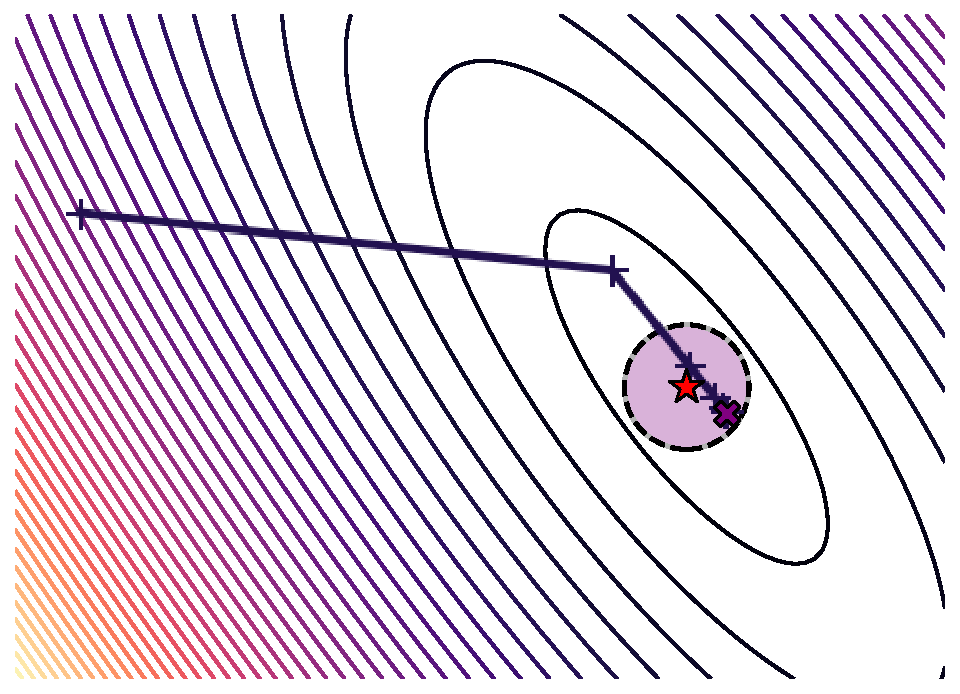
\includegraphics[width=0.3\linewidth]{images/plots/fedavg_True_10_t1000_s0.pdf}
  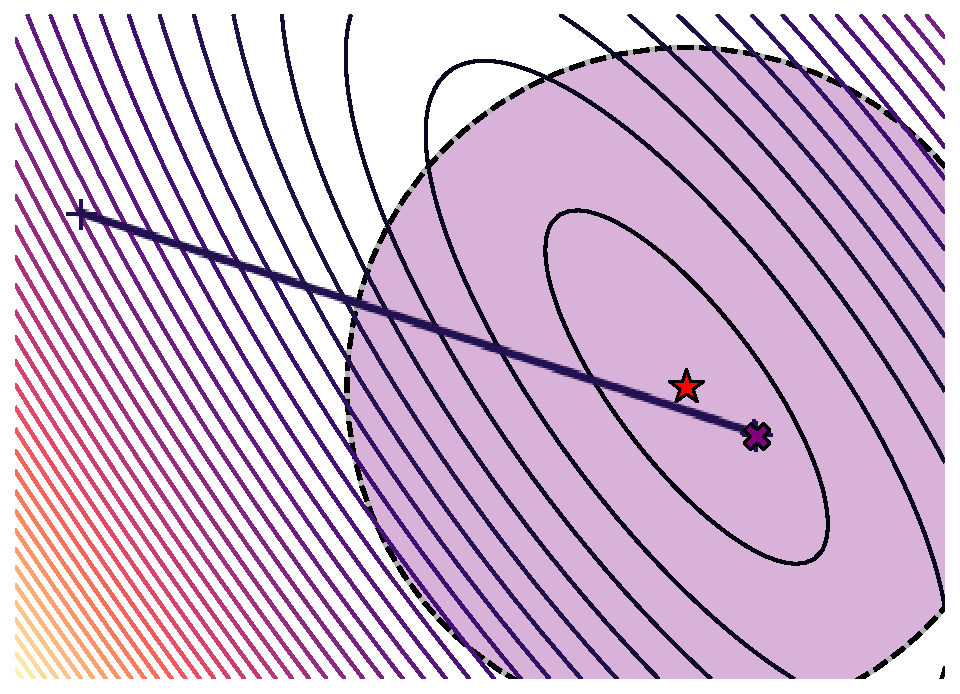
\includegraphics[width=0.3\linewidth]{images/plots/fedavg_True_50_t1000_s0.pdf}
}%
\only<4>{
  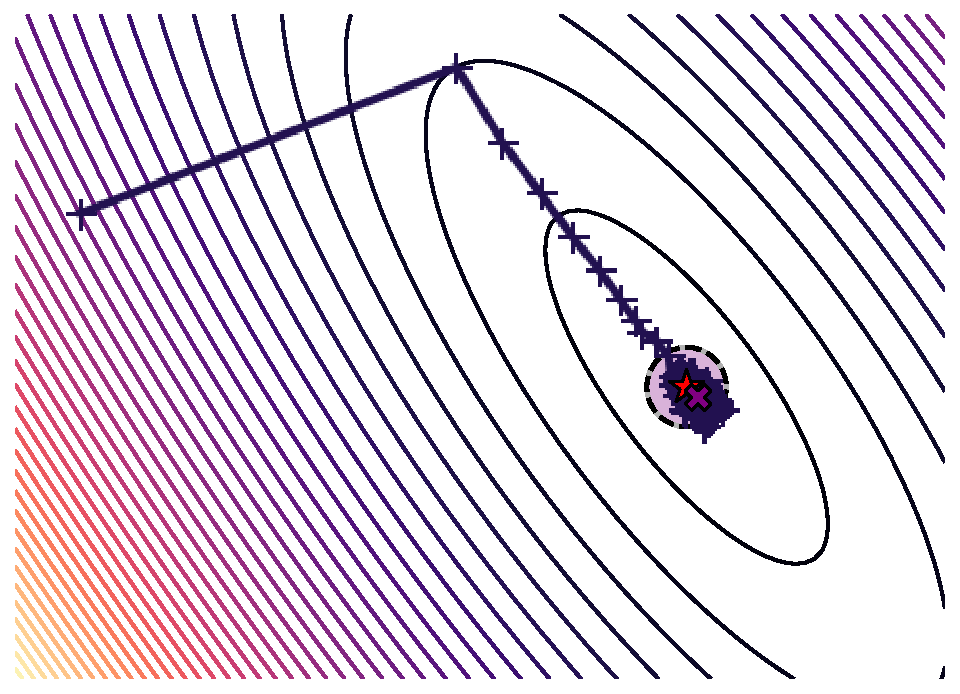
\includegraphics[width=0.3\linewidth]{images/plots/fedavg_True_2_t1000_s1.pdf}
  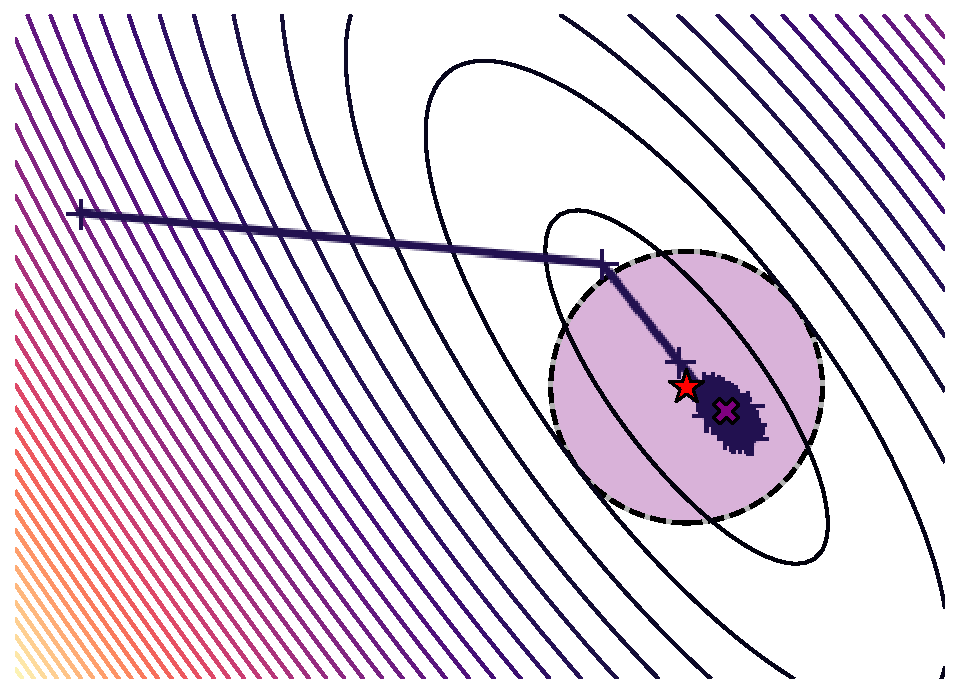
\includegraphics[width=0.3\linewidth]{images/plots/fedavg_True_10_t1000_s1.pdf}
  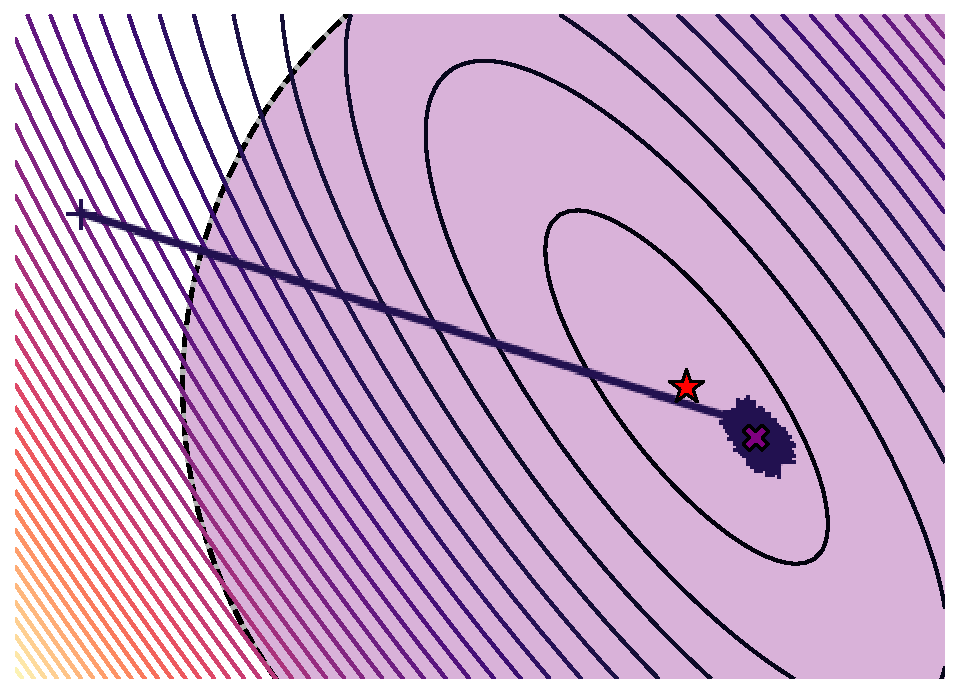
\includegraphics[width=0.3\linewidth]{images/plots/fedavg_True_50_t1000_s1.pdf}
}

  \end{center}

  \begin{center}
    When the number of local iterations increases, bias incrases

    \pause
    
    ... but the bound is oblivious to problem's geometry
    

  \pause
  
  \textcolor{purple}{\bfseries Remark:} It seems that iterates converge in some way?
  \end{center}
  
\end{frame}




\begin{frame}[t]{FedAvg (with stochastic gradients) converges!\footfullcite{mangold2025refined}\\[-0.5em]
      \small (For thrice derivable, $L$-smooth, $\mu$-strongly convex functions)}
    
\begin{itemize}[leftmargin=*]
    \item FedAvg converges to a stationary distribution $\pi^{(\gamma, H)}$
    \only<1>{
    \begin{itemize}
        \item denoting $x^{(t)} \sim \psi_{x^{(t)}}$, we have
    \begin{align*}
        \mathcal{W}_2(\psi_{x^{(t)}}; \pi^{(\gamma, H)})
        \le
        (1 - \gamma \mu)^{H t} \mathcal{W}_2(\psi_{x^{(0)}}; \pi^{(\gamma, H)})
    \end{align*}
    \item where $\mathcal{W}_2$ is the second order Wasserstein distance
    \end{itemize}
    }

\pause

    \item FedAvg's iterates covariance is
    \only<2,3>{
    \begin{align*}
    \int (x - x^\star)(x - x^\star)^\top \pi^{(\gamma, H)}(\mathrm{d} x)
    &  =
    \tikz[remember picture,baseline=(variance.base)] \node[pinkblock] (variance) at (0,0) {
    \textnormal{$\displaystyle \frac{\gamma}{N} C(x^\star) $}}; + O(\gamma^{3/2} H)
    \end{align*}
    }

\only<3>{
\begin{tikzpicture}[overlay,remember picture]
    \node[pinkblock] (variancelegend) at (5,4) {\shortstack{\underline{Linear speed-up !} \\[0.5em]
    variance decreases in $1/N$ \\
    variance scales in $\gamma$
    }};
    \draw[color=amethyst] (variance) -- (variancelegend);
\end{tikzpicture}

\vspace{-4em}
}
\pause

\pause


    \item We can now give an \textcolor{purple}{\bfseries exact expansion of the bias}
    \only<4,5>{
    \begin{align*}
    \int x \pi^{(\gamma, H)}(\mathrm{d} x)
    &  = x^\star +
    \tikz[remember picture,baseline=(heterbias.base)] \node[blueblock] (heterbias) at (0,0) {
    \textnormal{$\displaystyle \frac{\gamma (H-1)}{2N}
    \sum_{c=1}^N \nabla^2 f(x^\star)^{-1}
    \big( \nabla^2 f_c(x^\star) - \nabla^2 f(x^\star) \big)
    \nabla f_c(x^\star)$}
    };
    \\ 
    &  \qquad
    -  \tikz[remember picture,baseline=(stobias.base)] \node[pinkblock] (stobias) at (0,0) {
    \textnormal{$\displaystyle
    \frac{\gamma}{2 N} \nabla^2 f(x^\star)^{-1}
    \nabla^3 f(x^\star) A^{-1} C(x^\star)
    $}};
    + O(\gamma^{3/2} H)
    \end{align*}
    }
\pause

\only<4,5>{
\begin{tikzpicture}[overlay,remember picture]
    \node[blueblock] (heterbiaslegend) at (3,6) {\shortstack{\underline{Heterogeneity bias} \\[0.5em]
     vanishes when $\nabla^2 f_c(x^\star) = \nabla^2 f(x^\star)$ \\
    \quad or when $\nabla f_c(x^\star) = \nabla f(x^\star)$
    }};
    \draw[color=amethyst] (heterbias) -- (heterbiaslegend);
    
    \node[pinkblock] (stobiaslegend) at (10.5,6) {\shortstack{\underline{Stochasticity bias} \\[0.5em]
    $A$ is some linear operator \\
    $C(x^\star)$ is $\nabla f$'s covariance at $x^\star$
    }};
    \draw[color=amaranth] (stobias) -- (stobiaslegend);
\end{tikzpicture}

\vspace{-4em}
}

\end{itemize}

\vspace{4em}

\end{frame}



\begin{frame}
  \begin{center}
    \huge \textcolor{purple}{
      II. Correcting heterogeneity: Scaffold
      }
  \end{center}
\end{frame}


\begin{frame}[t]{Scaffold\footfullcite{karimireddy2020scaffold} ~~~ \raisebox{0.2em}{\textcolor{black}{\normalsize $x^\star \in \arg\min_{x \in \mathbb{R}^d} 
    \frac{1}{N} \sum_{c=1}^N \mathbb{E}_Z[ F_c(x; Z) ]$}} ~~}  
    
    \vspace{-1em}

  \begin{minipage}{0.5\linewidth}

  \footnotesize
  At each global iteration

    \begin{itemize}[leftmargin=*,itemsep=0em]
  \footnotesize
    \item For $c=1$ to $N$ in parallel

\vspace{-0.2em}
    
    
\begin{itemize}[leftmargin=*,itemsep=0em]
\item Receive $x^{(t)}$, set $x^{(t,0)}_c = x^{(t)}$
    
        \item For $h=0$ to $H-1$
    \end{itemize}

\vspace{-0.6em}
\begin{center}
            \hspace{-1em}$x^{(t,h+1)}_c = x^{(t,h)}_c - \gamma \big( \nabla F_c( x^{(t,h)}_c ; Z_c^{(t,h+1)}) + \textcolor{purple}{\boldsymbol{\xi_c^{(t)}}} \big)$
        \end{center}
      
  \item Aggregate models, update control variates
        
        
\vspace{-0.6em}
\begin{center}
            \hspace{-1em}$x^{(t+1)} = \frac{1}{N} \sum_{c=1}^N x_c^{(t,H)}$
          \end{center}
\begin{center}
            \hspace{-1em}$\textcolor{purple}{\boldsymbol{\xi_c^{(t+1)} = \xi_c^{(t)} + \frac{1}{\gamma H} (\theta_c^{t,H} - \theta^{(t+1)} )}}$
          \end{center}

          
      
    \end{itemize}
      
  \end{minipage}~~~~~~%
  \begin{minipage}{0.48\linewidth}
  \pause
       \begin{center}
    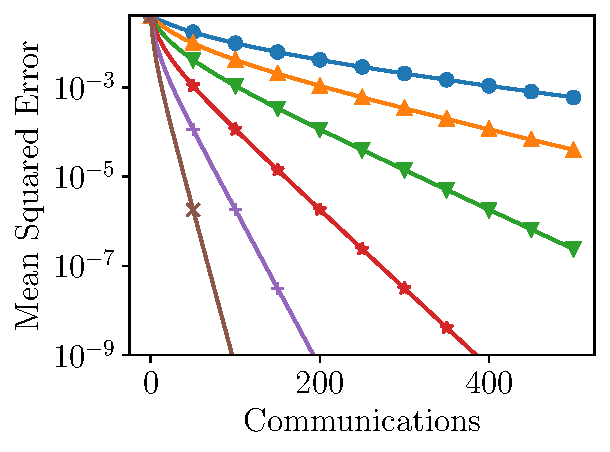
\includegraphics[width=0.75\linewidth]{images/local_training_homogeneous.pdf}%
    \raisebox{2.5em}{ 
\includegraphics[width=0.25\linewidth]{images/legend.pdf} }
  \end{center}
  
    \vspace{-0.5em}

  $\rightarrow$ No more heterogeneity bias!

  \end{minipage}

  \vspace{1.5em}


\end{frame}




\begin{frame}[t]{Scaffold also converges !\footfullcite{mangold2025scaffold}\\[-0.5em]
  \small (For $L$-smooth, $\mu$-strongly convex functions with $\nabla^3 f(x)$ bounded by $Q$)}


\begin{itemize}[leftmargin=*]
    \item Scaffold converges if $\gamma H L \le 1$, towards a distribution $\pi^{(\gamma, H)}$
    \only<1>{
    \begin{itemize}
        \item denoting $x^{(t)} \sim \psi_{x^{(t)}}$, we have
    \begin{align*}
        \mathcal{W}_2(\psi_{x^{(t)}}; \pi^{(\gamma, H)})
        \le
        (1 - \gamma \mu)^{H t} \mathcal{W}_2(\psi_{x^{(0)}}; \pi^{(\gamma, H)})
    \end{align*}
    \item where $\mathcal{W}_2$ is the second order Wasserstein distance
    \end{itemize}
    }

    \pause
    
  \item Scaffold's variance is close to FedAvg's variance
    \only<2,3>{
      \begin{align*}
        \int (x - x^\star)(x - x^\star)^\top \pi^{(\gamma, H)}(\mathrm{d} x)
        &  =
          \tikz[remember picture,baseline=(variance.base)] \node[pinkblock] (variance) at (0,0) {
          \textnormal{$\displaystyle \frac{\gamma}{N} C(x^\star) $}}; + O(\gamma^{3/2})
      \end{align*}
    }
    \pause
    
    \only<3>{
      \begin{tikzpicture}[overlay,remember picture]
        \node[pinkblock] (variancelegend) at (5,4) {\shortstack{\underline{Linear speed-up !} \\[0.5em]
            variance decreases in $1/N$ \\
            variance scales in $\gamma$
          }};
        \draw[color=amethyst] (variance) -- (variancelegend);
      \end{tikzpicture}
      
      \vspace{-4em}
    }

    \pause

  \item Scaffold still has some bias
    \only<4,5>{
      \begin{align*}
        \int x \pi^{(\gamma, H)}(\mathrm{d} x)
        &  = x^\star
          -  \tikz[remember picture,baseline=(stobias.base)] \node[pinkblock] (stobias) at (0,0) {
          \textnormal{$\displaystyle
          \frac{\gamma}{2 N} \nabla^2 f(x^\star)^{-1}
          \nabla^3 f(x^\star) A^{-1} C(x^\star)
          $}};
          + O(\gamma^{3/2})
      \end{align*}
    }

    \only<5>{
      \begin{tikzpicture}[overlay,remember picture]    
        \node[pinkblock] (stobiaslegend) at (10.5,4) {\shortstack{\underline{Stochasticity bias remains!} \\[0.5em]
            $A$ is some linear operator \\
            $C(x^\star)$ is $\nabla f$'s covariance at $x^\star$
          }};
        \draw[color=amaranth] (stobias) -- (stobiaslegend);
      \end{tikzpicture}

      \vspace{-4em}
    }

\pause

\end{itemize}

\end{frame}
\begin{frame}[t]
  \begin{center}
    
  \resizebox{0.9\linewidth}{!}{
  \begin{tikzpicture}
    \draw [-to,very thick](0,0) -- (12.5,0);
    \node at (1.5,0.2) {$H=10$};
    \node at (6,0.2) {$H=20$};
    \node at (10.5,0.2) {$H=50$};
  \end{tikzpicture}
}
\vspace{-0.5em}

\only<1>{
  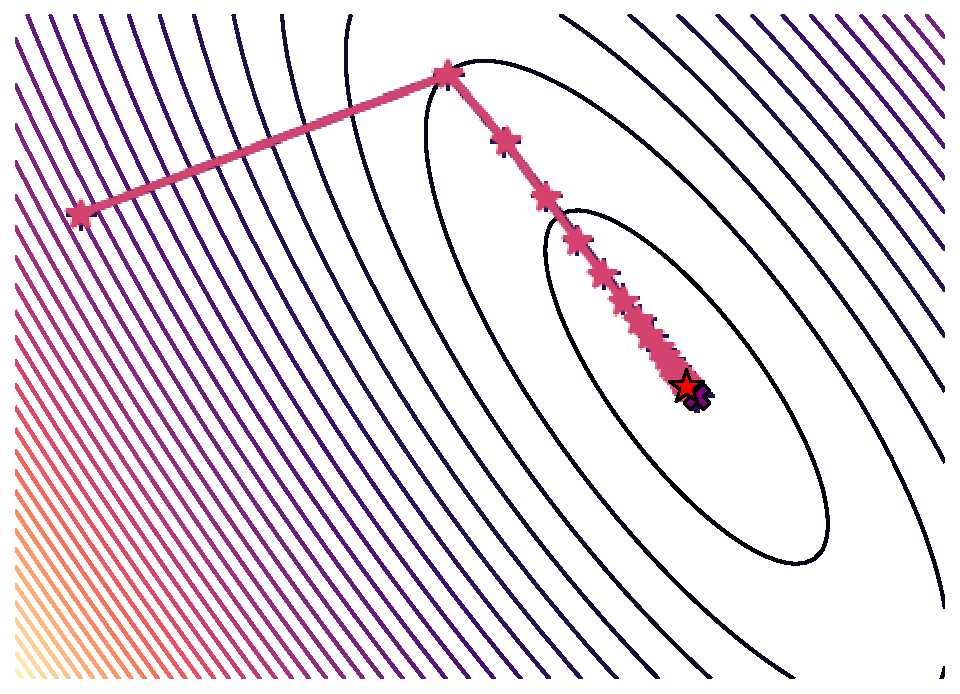
\includegraphics[width=0.3\linewidth]{images/plots/fedavg_scaffold_True_2_t1000_s0.pdf}
  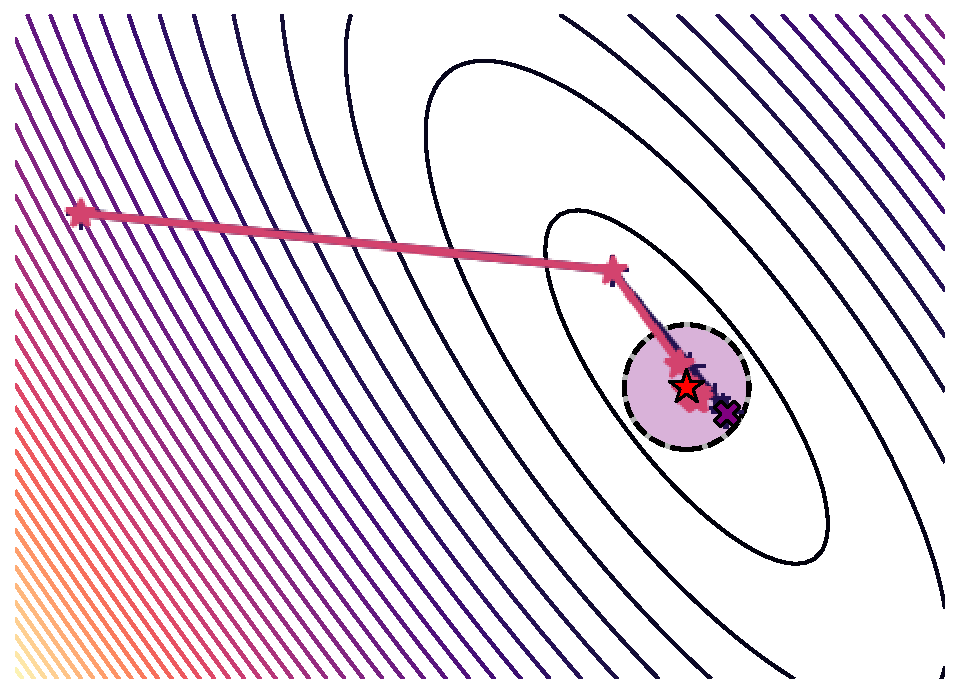
\includegraphics[width=0.3\linewidth]{images/plots/fedavg_scaffold_True_10_t1000_s0.pdf}
  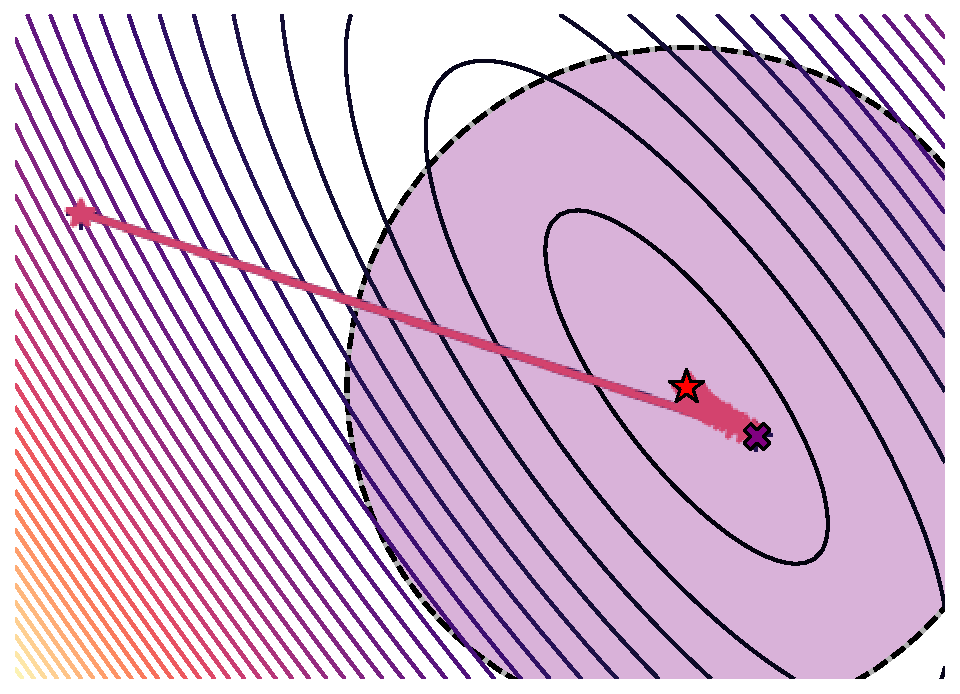
\includegraphics[width=0.3\linewidth]{images/plots/fedavg_scaffold_True_50_t1000_s0.pdf}
}%
\only<2>{
  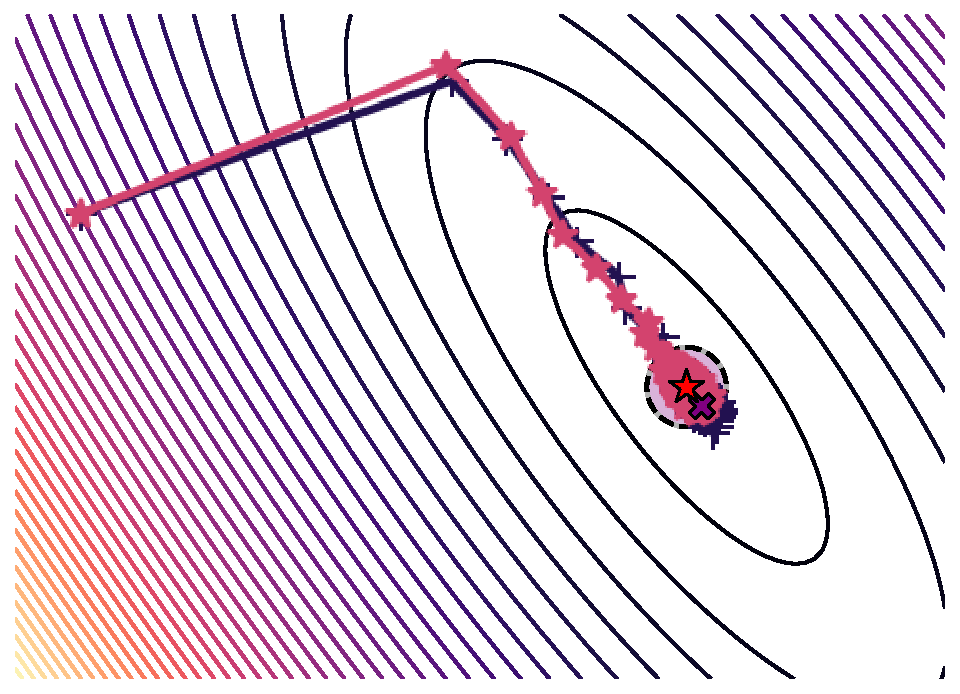
\includegraphics[width=0.3\linewidth]{images/plots/fedavg_scaffold_True_2_t1000_s1.pdf}
  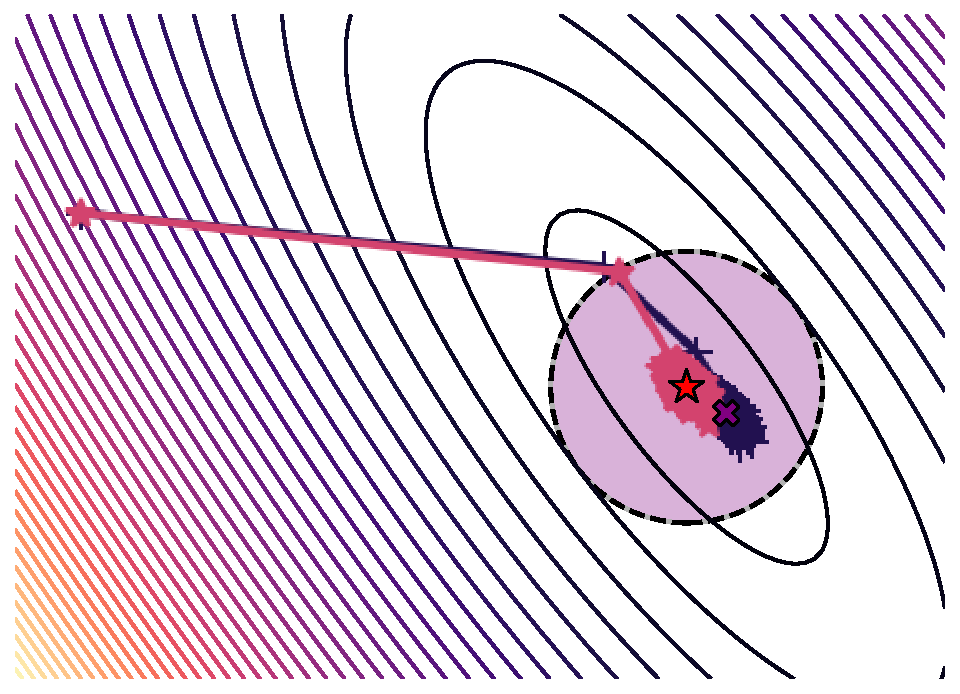
\includegraphics[width=0.3\linewidth]{images/plots/fedavg_scaffold_True_10_t1000_s1.pdf}
  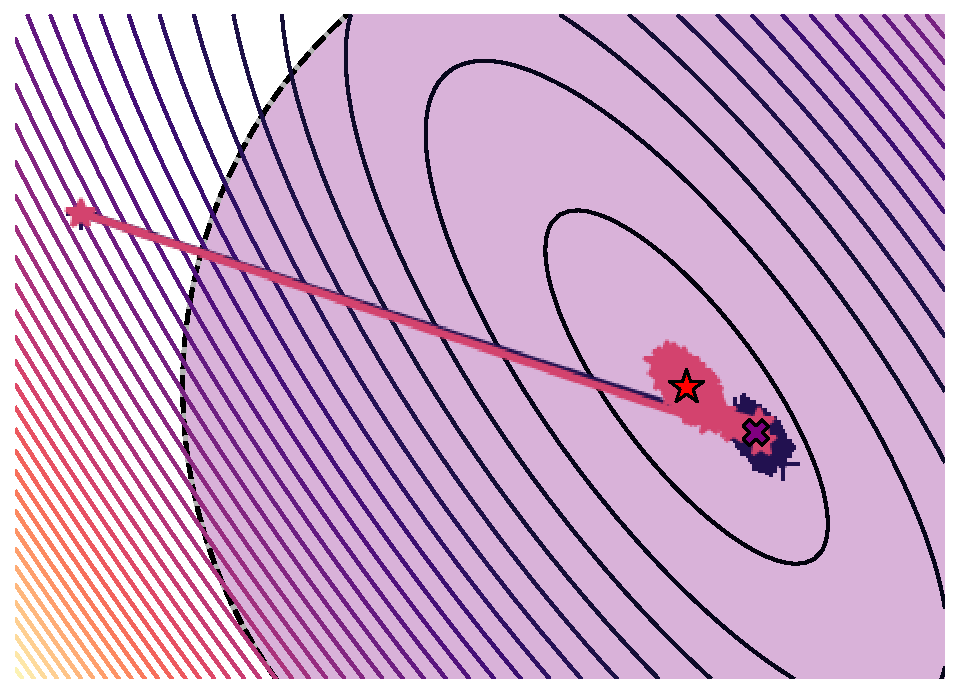
\includegraphics[width=0.3\linewidth]{images/plots/fedavg_scaffold_True_50_t1000_s1.pdf}
}

  \end{center}

  \begin{center}
    Scaffold converges to the right point


    ... and its variance is similar to FedAvg!
  \end{center}


\end{frame}


\begin{frame}{New Convergence Rate for Scaffold\\[-0.5em]
    \small (For $L$-smooth, $\mu$-strongly convex functions with $\nabla^3 f(x)$ bounded by $Q$)}
\begin{align*}
\mathbb{E}\left[ \| x^{(T)} - x^\star \|^2 \right] 
& \lesssim{} \left( 1 - \frac{\gamma \mu}{4} \right)^{HT}
\left\{ 
\| x^{(0)} - x^\star \|^2
+
2\gamma^2 H^2 \zeta^2
+
\frac{ \sigma_\star^2 }{L\mu}
\right\}
\\ &  \quad\quad\quad\quad\quad\quad\quad
+ 
\frac{\gamma }{\textcolor{purple}{\boldsymbol{N}} \mu} \sigma_\star^2 
+ \frac{ \gamma^{3/2} Q }{\mu^{5/2}} \sigma_\star^3
+ \frac{ \gamma^3 H Q^2}{\mu^3} \sigma_\star^4
\end{align*}


where
\begin{itemize}
\item \small
  $\sigma_\star^2 = \mathbb{E}[ \frac{1}{N} \sum_{c=1}^N \| \nabla F_c^Z(x^\star) - \nabla f_c(x^\star) \|^2$ is the variance at $x^\star$
\item \small
  $\zeta^2 = \frac{1}{N} \sum_{c=1}^N \| \nabla f_c^Z(x^\star) \|^2$ measures gradient heterogeneity
\end{itemize}



\end{frame}

\begin{frame}{Linear Speed-Up!}

  As long as $N$ is not too large, one can obtain $\mathbb{E}\left[ \| x^{(T)} - x^\star \|^2 \right] \le \epsilon^2 $ with
  \begin{align*}
    \# \text{grad per client}
    = \widetilde O\Big( \frac{\sigma_\star^2}{\textcolor{purple}{\boldsymbol{N}} \mu^2 \epsilon^2} 
    \log\left( 
    \frac{1}{\epsilon}
    \right) \Big)
  \end{align*}
  
\end{frame}

\begin{frame}{Conclusion}

  \begin{itemize}[itemsep=1em]
  \item FedAvg and Scaffold converge (even with stochastic gradients)
  \item This allows to derive new analyses for these problems,

    with exact first-order expression for bias
  \item And we proved that Scaffold has:
    \begin{itemize}
    \item variance similar to FedAvg's variance
    \item \textit{linear speed-up} in the number of clients!!
    \end{itemize}

  \end{itemize}
  
\end{frame}


\end{document}
%%% Local Variables:
%%% mode: latex
%%% TeX-master: t
%%% End:
